\documentclass[a4paper,12pt]{article}
\usepackage[margin=18mm]{geometry}
\usepackage{tikz}
\usepackage{amsmath}
\usepackage{xcolor}
\newcommand{\pFourCell}[2]{\makebox[#1em][c]{\ensuremath{#2}}}
\newcommand{\pFourCenterBox}[1]{\begingroup\setbox0=\hbox{$\displaystyle #1$}\dimen0=\ht0\advance\dimen0 by -\dp0\divide\dimen0 by 2\lower\dimen0\box0\endgroup}
\newdimen\pFourFractionRuleThickness
\pFourFractionRuleThickness=0.4pt
\newcommand{\pFourTopAlign}[3]{\raisebox{-#1}[0pt][\dimexpr #1 + #2\relax]{\ensuremath{\displaystyle #3}}}
\newcommand{\pFourBottomAlign}[3]{\raisebox{#2}[\dimexpr #1 + #2\relax][0pt]{\ensuremath{\displaystyle #3}}}
\newcommand{\pFourFractionInner}[2]{\hbox to #1{\hss$\displaystyle #2$\hss}}
\newcommand{\pFourFractionC}[4]{\begingroup\color{#1}\genfrac{}{}{\pFourFractionRuleThickness}{0}{\raisebox{0.14em}{\pFourFractionInner{#2}{{\color{black}#3}}}}{\raisebox{-0.18em}{\pFourFractionInner{#2}{{\color{black}#4}}}}\endgroup}
\newcommand{\pFourFraction}[3]{\genfrac{}{}{\pFourFractionRuleThickness}{0}{\raisebox{0.14em}{\pFourFractionInner{#1}{#2}}}{\raisebox{-0.18em}{\pFourFractionInner{#1}{#3}}}}
\newcommand{\pFourRootC}[2]{\begingroup\setbox0=\hbox{$\displaystyle #2$}\setbox2=\hbox{$\displaystyle \sqrt{\phantom{\copy0}}$}\dimen0=\wd2\advance\dimen0 by -\wd0\hbox{\rlap{\textcolor{#1}{\copy2}}\kern\dimen0\box0}\endgroup}
\newcommand{\pFourRoot}[1]{\pFourRootC{black}{#1}}
\newcommand{\pFourRootDegreeC}[3]{\begingroup\setbox0=\hbox{$\displaystyle #3$}\setbox2=\hbox{$\displaystyle \sqrt[#2]{\phantom{\copy0}}$}\dimen0=\wd2\advance\dimen0 by -\wd0\hbox{\rlap{\textcolor{#1}{\copy2}}\kern\dimen0\box0}\endgroup}
\newcommand{\pFourRootDegree}[2]{\pFourRootDegreeC{black}{#1}{#2}}
\pagestyle{empty}
\begin{document}

\section*{Spaltentreue LaTeX-Ausgabe}
\noindent Gleichung: \texttt{a}\texttt{/}\texttt{sin}\texttt{(}\ensuremath{\alpha}\texttt{)=}\texttt{b}\texttt{/}\texttt{sin}\texttt{(}\ensuremath{\beta}\texttt{)} \hfill Zielvariable: \ensuremath{\alpha} \hfill Profil: \texttt{standard}

\vspace{8mm}
\begin{center}
\begin{tikzpicture}[x=1em,y=-1em]
\node[anchor=base, inner sep=0pt] at (10.524,2.88) {$\pFourFraction{3.68em}{\pFourCell{3.68}{a}}{\pFourCell{3.68}{\sin\left(\alpha\right)}}$};
\node[anchor=base, inner sep=0pt] at (16.538,2.88) {$\pFourCell{1.62}{=}$};
\node[anchor=base, inner sep=0pt] at (21.118,2.88) {$\pFourFraction{3.77em}{\pFourCell{3.77}{b}}{\pFourCell{3.77}{\sin\left(\beta\right)}}$};
\node[anchor=base, inner sep=0pt] at (14.204,7.73) {$\pFourCell{0.9}{a}$};
\node[anchor=base, inner sep=0pt] at (16.538,7.73) {$\pFourCell{1.62}{=}$};
\node[anchor=base, inner sep=0pt] at (23.018,7.73) {$\pFourFraction{3.77em}{\pFourCell{3.77}{b}}{\pFourCell{3.77}{\sin\left(\beta\right)}}\sin\left(\alpha\right)$};
\node[anchor=base, inner sep=0pt] at (12.364,12.58) {$\pFourFraction{3.68em}{\pFourCell{3.68}{a}}{\pFourTopAlign{0.95em}{1.14em}{\pFourFraction{3.68em}{\pFourCell{3.68}{b}}{\pFourCell{3.68}{\sin\left(\beta\right)}}}}$};
\node[anchor=base, inner sep=0pt] at (16.538,12.58) {$\pFourCell{1.62}{=}$};
\node[anchor=base, inner sep=0pt] at (27.788,12.58) {$\pFourCell{4.58}{\sin\left(\alpha\right)}$};
\node[anchor=base, inner sep=0pt] at (8.684,20.34) {$\pFourCell{15.728}{\operatorname{asin}\left(\pFourFraction{3.68em}{\pFourCell{3.68}{a}}{\pFourTopAlign{0.95em}{1.14em}{\pFourFraction{3.68em}{\pFourCell{3.68}{b}}{\pFourCell{3.68}{\sin\left(\beta\right)}}}}\right)}$};
\node[anchor=base, inner sep=0pt] at (16.538,20.34) {$\pFourCell{1.62}{=}$};
\node[anchor=base, inner sep=0pt] at (28.238,20.34) {$\pFourCell{0.9}{\alpha}$};
\end{tikzpicture}
\end{center}


\newpage
\section*{Spaltentreue LaTeX-Ausgabe mit Spaltengrenzen}
\vspace{6mm}
\begin{center}
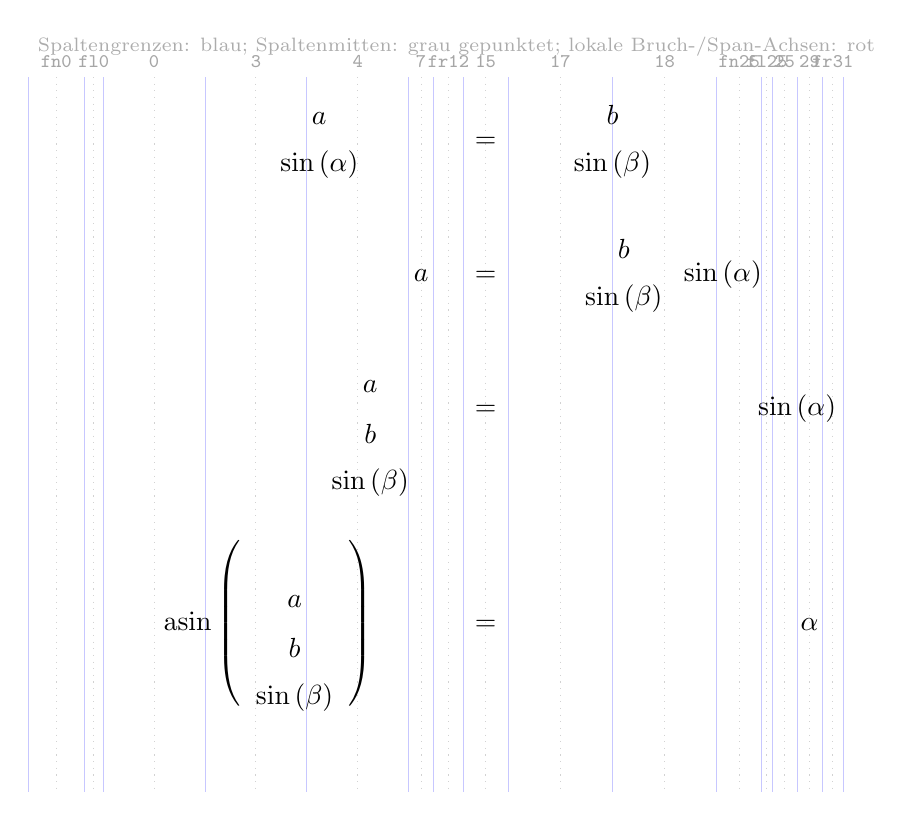
\begin{tikzpicture}[x=1em,y=-1em]
\node[font={\scriptsize}, text=gray!65, anchor=west] at (0,-0.75) {Spaltengrenzen: blau; Spaltenmitten: grau gepunktet; lokale Bruch-/Span-Achsen: rot};
\draw[blue!22, line width=0.28pt] (0,0.35) -- (0,26.17);
\draw[blue!22, line width=0.28pt] (2.04,0.35) -- (2.04,26.17);
\draw[blue!22, line width=0.28pt] (2.714,0.35) -- (2.714,26.17);
\draw[blue!22, line width=0.28pt] (6.394,0.35) -- (6.394,26.17);
\draw[blue!22, line width=0.28pt] (10.074,0.35) -- (10.074,26.17);
\draw[blue!22, line width=0.28pt] (13.754,0.35) -- (13.754,26.17);
\draw[blue!22, line width=0.28pt] (14.654,0.35) -- (14.654,26.17);
\draw[blue!22, line width=0.28pt] (15.728,0.35) -- (15.728,26.17);
\draw[blue!22, line width=0.28pt] (17.348,0.35) -- (17.348,26.17);
\draw[blue!22, line width=0.28pt] (21.118,0.35) -- (21.118,26.17);
\draw[blue!22, line width=0.28pt] (24.888,0.35) -- (24.888,26.17);
\draw[blue!22, line width=0.28pt] (26.508,0.35) -- (26.508,26.17);
\draw[blue!22, line width=0.28pt] (26.888,0.35) -- (26.888,26.17);
\draw[blue!22, line width=0.28pt] (27.788,0.35) -- (27.788,26.17);
\draw[blue!22, line width=0.28pt] (28.688,0.35) -- (28.688,26.17);
\draw[blue!22, line width=0.28pt] (29.468,0.35) -- (29.468,26.17);
\draw[gray!35, dotted] (1.02,0.35) -- (1.02,26.17);
\node[font={\ttfamily\scriptsize}, text=gray!70, anchor=base] at (1.02,0) {fn0};
\draw[gray!35, dotted] (2.377,0.35) -- (2.377,26.17);
\node[font={\ttfamily\scriptsize}, text=gray!70, anchor=base] at (2.377,0) {fl0};
\draw[gray!35, dotted] (4.554,0.35) -- (4.554,26.17);
\node[font={\ttfamily\scriptsize}, text=gray!70, anchor=base] at (4.554,0) {0};
\draw[gray!35, dotted] (8.234,0.35) -- (8.234,26.17);
\node[font={\ttfamily\scriptsize}, text=gray!70, anchor=base] at (8.234,0) {3};
\draw[gray!35, dotted] (11.914,0.35) -- (11.914,26.17);
\node[font={\ttfamily\scriptsize}, text=gray!70, anchor=base] at (11.914,0) {4};
\draw[gray!35, dotted] (14.204,0.35) -- (14.204,26.17);
\node[font={\ttfamily\scriptsize}, text=gray!70, anchor=base] at (14.204,0) {7};
\draw[gray!35, dotted] (15.191,0.35) -- (15.191,26.17);
\node[font={\ttfamily\scriptsize}, text=gray!70, anchor=base] at (15.191,0) {fr12};
\draw[gray!35, dotted] (16.538,0.35) -- (16.538,26.17);
\node[font={\ttfamily\scriptsize}, text=gray!70, anchor=base] at (16.538,0) {15};
\draw[gray!35, dotted] (19.233,0.35) -- (19.233,26.17);
\node[font={\ttfamily\scriptsize}, text=gray!70, anchor=base] at (19.233,0) {17};
\draw[gray!35, dotted] (23.003,0.35) -- (23.003,26.17);
\node[font={\ttfamily\scriptsize}, text=gray!70, anchor=base] at (23.003,0) {18};
\draw[gray!35, dotted] (25.698,0.35) -- (25.698,26.17);
\node[font={\ttfamily\scriptsize}, text=gray!70, anchor=base] at (25.698,0) {fn25};
\draw[gray!35, dotted] (26.698,0.35) -- (26.698,26.17);
\node[font={\ttfamily\scriptsize}, text=gray!70, anchor=base] at (26.698,0) {fl25};
\draw[gray!35, dotted] (27.338,0.35) -- (27.338,26.17);
\node[font={\ttfamily\scriptsize}, text=gray!70, anchor=base] at (27.338,0) {25};
\draw[gray!35, dotted] (28.238,0.35) -- (28.238,26.17);
\node[font={\ttfamily\scriptsize}, text=gray!70, anchor=base] at (28.238,0) {29};
\draw[gray!35, dotted] (29.078,0.35) -- (29.078,26.17);
\node[font={\ttfamily\scriptsize}, text=gray!70, anchor=base] at (29.078,0) {fr31};
\node[anchor=base, inner sep=0pt] at (10.524,2.88) {$\pFourFraction{3.68em}{\pFourCell{3.68}{a}}{\pFourCell{3.68}{\sin\left(\alpha\right)}}$};
\node[anchor=base, inner sep=0pt] at (16.538,2.88) {$\pFourCell{1.62}{=}$};
\node[anchor=base, inner sep=0pt] at (21.118,2.88) {$\pFourFraction{3.77em}{\pFourCell{3.77}{b}}{\pFourCell{3.77}{\sin\left(\beta\right)}}$};
\node[anchor=base, inner sep=0pt] at (14.204,7.73) {$\pFourCell{0.9}{a}$};
\node[anchor=base, inner sep=0pt] at (16.538,7.73) {$\pFourCell{1.62}{=}$};
\node[anchor=base, inner sep=0pt] at (23.018,7.73) {$\pFourFraction{3.77em}{\pFourCell{3.77}{b}}{\pFourCell{3.77}{\sin\left(\beta\right)}}\sin\left(\alpha\right)$};
\node[anchor=base, inner sep=0pt] at (12.364,12.58) {$\pFourFraction{3.68em}{\pFourCell{3.68}{a}}{\pFourTopAlign{0.95em}{1.14em}{\pFourFraction{3.68em}{\pFourCell{3.68}{b}}{\pFourCell{3.68}{\sin\left(\beta\right)}}}}$};
\node[anchor=base, inner sep=0pt] at (16.538,12.58) {$\pFourCell{1.62}{=}$};
\node[anchor=base, inner sep=0pt] at (27.788,12.58) {$\pFourCell{4.58}{\sin\left(\alpha\right)}$};
\node[anchor=base, inner sep=0pt] at (8.684,20.34) {$\pFourCell{15.728}{\operatorname{asin}\left(\pFourFraction{3.68em}{\pFourCell{3.68}{a}}{\pFourTopAlign{0.95em}{1.14em}{\pFourFraction{3.68em}{\pFourCell{3.68}{b}}{\pFourCell{3.68}{\sin\left(\beta\right)}}}}\right)}$};
\node[anchor=base, inner sep=0pt] at (16.538,20.34) {$\pFourCell{1.62}{=}$};
\node[anchor=base, inner sep=0pt] at (28.238,20.34) {$\pFourCell{0.9}{\alpha}$};
\end{tikzpicture}
\end{center}
\end{document}
